\chapter{Berechenbarkeitstheorie}
\begin{center}
	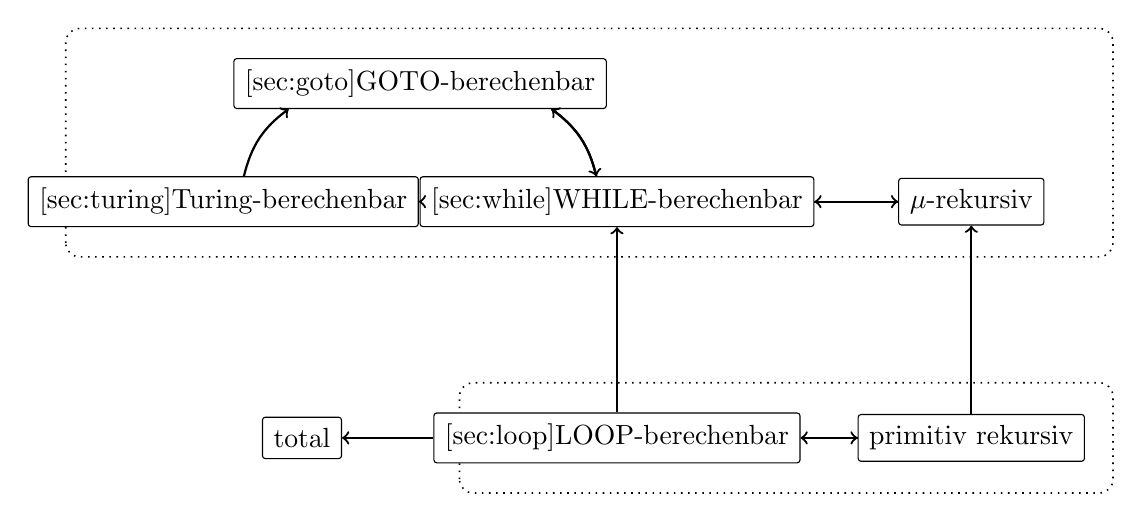
\begin{tikzpicture}
		\tikzset{
			grouplabel/.style={
				draw,
				fill = white,
				rectangle,
				inner sep = 4pt,
				rounded corners=1pt
			}
		}

		\draw [rounded corners=5pt, dotted, line width=0.2mm] (0,6.3) rectangle (13.3,9.2);
		\draw node (tm) at (2,7) [grouplabel] {\hyperref[sec:turing]{Turing-berechenbar}};
		\draw node (while) at (7,7) [grouplabel] {\hyperref[sec:while]{WHILE-berechenbar}};
		\draw node (goto) at (4.5,8.5) [grouplabel] {\hyperref[sec:goto]{GOTO-berechenbar}};
		\draw node (mu) at (11.5,7) [grouplabel] {$\mu$-rekursiv};
		\draw [rounded corners=5pt, dotted, line width=0.2mm] (5,3.3) rectangle (13.3,4.7);
		\draw node (loop) at (7,4) [grouplabel] {\hyperref[sec:loop]{LOOP-berechenbar}};
		\draw node (prek) at (11.5,4) [grouplabel] {primitiv rekursiv};
		\draw node (total) at (3,4) [grouplabel] {total};

		\draw[thick, ->] (while) to (tm);
		\draw[thick, ->] (tm) to[bend left=20] (goto);
		\draw[thick, ->] (goto) to[bend left=20] (while);
		\draw[thick, ->] (while) to[bend right=20] (goto);
		\draw[thick, ->] (mu) to (while);
		\draw[thick, ->] (while) to (mu);

		\draw[thick, ->] (prek) to (mu);
		\draw[thick, ->] (loop) to (while);
		\draw[thick, ->] (loop) to (prek);
		\draw[thick, ->] (prek) to (loop);

		\draw[thick, ->] (loop) to (total);
	\end{tikzpicture}
\end{center}




\section{LOOP-Berechenbarkeit}\label{sec:loop}
Eine Funktion $f:\N^k\rightarrow \N$ heißt LOOP-berechenbar,  falls es ein LOOP-Program $P$ gibt, das gestartet auf der Eingabe $n_1,n_2,\ldots,n_k$ in den Variablen $x_1,x_2,\ldots,x_n$ nach endlich vielen Schritten hält und die Variable $x_0$ den Wert $f(n_1,\ldots,n_k)$ beinhaltet.
\subsection{Erlaubte Basisanweisungen}
\begin{itemize}
	\item $x_i\coloneqq x_j+c$ bzw. $x_i\coloneqq x_j-c$ mit $c\in\N$
	\item LOOP $x_i$ DO $P$ END
	\item Hintereinanderausführung
\end{itemize}
\subsection{Simulierbare Makros}
\begin{itemize}
	\item Wertzuweisungen $x_i\coloneqq x_j$ und $x_i\coloneqq c$
	\item IF $x_i>c$ THEN $P$ END
	\item Übliche Arithmetische Operationen (Multiplikation und Division), sogar $\mathrm{mod}$
\end{itemize}

\section{WHILE-Berechenbarkeit}\label{sec:while}
Eine Funktion $f:\N^k\rightarrow \N$ heißt WHILE-berechenbar,  falls es ein WHILE-Program $P$ gibt, das gestartet auf der Eingabe $n_1,n_2,\ldots,n_k$ in den Variablen $x_1,x_2,\ldots,x_n$ nach endlich vielen Schritten hält (falls das Ergebnis definiert ist) und die Variable $x_0$ den Wert $f(n_1,\ldots,n_k)$ beinhaltet. Ist $f(n_1,\ldots,n_k)$ undefiniert, so hält $P$ nicht.
\subsection{Erlaubte Anweisungen}
\begin{itemize}
	\item In WHILE-Programmen sind alle Anweisungen von LOOP-Programmen erlaubt sowie die WHILE-Schleife:

	\item WHILE $x_i\neq 0$ DO $P$ END
\end{itemize}


\section{GOTO-Berechenbarkeit}\label{sec:goto}
\subsection{Erlaubte Anweisungen}
\begin{itemize}
	\item Berechnungen und Zuweisungen: $x_i\coloneqq x_j\pm c$
	\item Marken: $M_i$
	\item GOTO $M_i$
	\item HALT
	\item IF $x_i=c$ THEN GOTO $M_j$
\end{itemize}

\section{Turing-Berechenbarkeit}\label{sec:turing}
Eine Funktion $f:\N^k\rightarrow \N$ heißt Turing-berechenbar, falls eine deterministische Turingmaschine existiert, die $f(n_1,\ldots,n_k)=m$ berechnet indem, sie gestartet auf dem $k$-Tupel $(n_1,\ldots,n_k)$ nach endlich vielen Berechnungsschritten einen Endzustand erreicht und dann $m$ auf dem Band steht. Falls das Ergebnis für die Eingabe undefiniert ist, terminiert die Maschine nie.

\section{Primitive Rekursion}
Eine Funktion ist genau dann primitiv rekursiv, wenn sie LOOP-berechenbar ist.
\begin{itemize}
	\item Konstante Funktionen sind primitiv rekursiv
	\item Projektionen sind primitiv rekursiv
	\item Die Nachfolgerfunktion $s:\N\rightarrow\N, n\mapsto n+1$ ist primitiv rekursiv
	\item Verkettungen von primitiv rekursiven Funktionen sind primitiv rekursiv
	\item Funktionen, die durch primitive Rekursion aus primitiv rekursiven Funktionen entstehen, sind primitiv rekursiv:
	\begin{align*}
		f(0,x_1,\ldots,x_k)&=g(x_1,\ldots,x_k)\\
		f(n+1,x_1,\ldots,x_k)&=h(f(n,x_1,\ldots,x_k),n,x_1,\ldots,x_k)
	\end{align*}
	Das heißt, $g, h$ primitiv rekursiv $\Rightarrow$ $f$ primitiv rekursiv.
\end{itemize}
\subsection{Beispiele für primitiv rekursive Funktionen:}
\begin{itemize}
	\item Cantor'sche Paarungsfunktion
	\begin{align*}
		&c(x,y)=\binom{x+y+1}{2}+x \quad\text{ (bijektiv)}
		\intertext{mit den Umkehrungsfunktionen}
		&e(c(x,y))=x\text{ und }f(c(x,y))=y
	\end{align*}
	\item
\end{itemize}

\section{$\mu$-Rekursion}
\begin{equation*}
	\mu f(x_1,\ldots,x_k)=\min \set{n\in\N}{f(n,x_1,\ldots,x_k)=0 \wedge \forall m<n:f(m,x_1,\ldots,x_k)>0}
\end{equation*}
Der $\mu$-Operator liefert den kleinsten Eingabewert $n$ der ersten Variable, bei der die Funktion $0$ ausgibt. Dabei muss insbesondere $f$ für alle Werte kleiner als $n$ definiert sein, da sonst eine Berechnung nicht möglich wäre.

\begin{satz}{Satz von Kleene}
	Sei $f:\N^n\rightarrow\N$ eine $\mu$-rekursive Funktion. Dann existieren zwei $(n+1)$-stellige primitiv rekursive Funktionen $p$ und $q$ mit
	\begin{equation*}
		f(x_1,\ldots,x_n)=p(x_1,\ldots,x_n,\mu q(x_1,\ldots,x_n))
	\end{equation*}
\end{satz}
